\documentclass[conference,10pt]{IEEEtran}

% *** CITATION PACKAGES ***
\usepackage{cite}
%\usepackage[subtle]{savetrees}

% *** GRAPHICS RELATED PACKAGES ***
\ifCLASSINFOpdf
   \usepackage[pdftex]{graphicx}
   \graphicspath{{../pdf/}{../jpeg/}{./figures/}{./plots}}
   \DeclareGraphicsExtensions{.pdf,.jpeg,.png}
\else
   \usepackage[dvips]{graphicx}
   \graphicspath{{./figures/}{./plots}}
   \DeclareGraphicsExtensions{.eps}
\fi

%\usepackage{hyperref}
\usepackage[cmex10]{amsmath}
\usepackage[caption=false,font=footnotesize]{subfig}
\usepackage{url}
\usepackage{fixltx2e}
\usepackage{colortbl}
\usepackage{color}
\usepackage{xspace}
%\usepackage{randtext}
%\usepackage{subfigure}
\usepackage{tablefootnote}
%\usepackage{comment}
\usepackage{alltt}
\usepackage{multirow}
\usepackage[nolist]{acronym}
%\usepackage{subfigure}
\usepackage{caption}
%\usepackage{booktabs}
%\usepackage{tabularx,ragged2e,booktabs,caption}
%\usepackage{microtype}
\usepackage{hyphenat}
\usepackage[T1]{fontenc}
\usepackage{xcolor, soul}
\usepackage{listings}
\lstset{
basicstyle=\small\ttfamily,
columns=flexible,
breaklines=true
}
\usepackage{comment}
%Savetrees magic, ask Ryan about this before uncommenting, it buys you more space for text/figures but can be tricky to use and get your paper rejected if you don't use it properly
\usepackage[all=normal,paragraphs=tight,wordspacing=tight,charwidths=tight,indent=tight,floats=tight,leading=tight,lists=tight,bibnotes=normal]{savetrees}

\setlength{\parskip}{1.7pt}
\setlength\belowcaptionskip{10pt}
\newcommand{\cus}[1]{\textcolor{blue}{[cushorts: #1]}}
\newcommand{\ttz}[1]{\textcolor{purple}{[ttaraz: #1]}}
\newcommand{\reg}[1]{\textcolor{purple}{[reg: #1]}}
%use commands like doubleblind to hide text that might reveal your identity for double blind reviews (not as common as single blind), later when you have the final version you can upcate the command and bring back the text
\newcommand{\doubleblind}[1]{{#1}}

\newcommand{\refpend}[0]{\textcolor{red}{[Reference Needed]}}

%%%%%%%%%%%%%%%%%%%%% Start of Report %%%%%%%%%%%%%%%%%%%%%

\title{ELEC 876 Final Report - Graphical\\Analyses of HPC Middleware Libraries}
\author{
\IEEEauthorblockN{Curtis Shorts\\}
\IEEEauthorblockA{Electrical and Computer Engineering Department, Queen's University\\
11 Union Street, Kingston, Ontario, Canada\\
Email: {curtis.shorts@queensu.ca}}
%\vspace{-10pt}

%You need to include this if we're working with folks from Sanida in the US, otherwise don't uncomment this!
%\thanks{*Sandia National Laboratories is a multimission laboratory managed and operated by National Technology and Engineering Solutions of Sandia LLC, a wholly owned subsidiary of Honeywell International Inc. for the U.S. Department of Energy’s National Nuclear Security Administration under contract DE-NA0003525.}\\
}

% For how much blank space to remove after figures
%\newcommand\figrmspace{-15pt}

\IEEEoverridecommandlockouts

\begin{document}
%\input{cover_letter}

\maketitle

\begin{abstract}
%\cus{200 word limit}
High Performance Computing (HPC) communication libraries utilize network middleware libraries in order to minimize the latency experienced when interacting with the networking hardware that makes large-scale cluster computing possible. The issue for new developers of these middleware libraries is that they have little-to-no developer-level documentation on their architectures and are written in C, the semantics of which can make them difficult to interpret at a high level. This paper proposes a methodology for analyzing the architecture of HPC middleware libraries by parsing the source-code to form a weighted dependency graph, then extracting the libraries' architecture with clustering algorithms. The parsing techniques used in this work use a combination of regular expressions (RegEx) and ANTLR, a parser generation tool. RegEx and ANTLR allowed for simple detection of pre-processor declarations (i.e. macros) and context-dependent usage of more complex dependencies (e.g. functions and structs) respectively. The results presented in this work showed the dependency graphs, but not the clustering of the graphs, to be useful in analyzing the source-code of such libraries through developing an initial intuition as to key architectural features.
\end{abstract}


\section{Introduction and Background}
\label{sec:intro}

% Background on HPC nework library design
High Performance Computing (HPC) is the use of many compute nodes in parallel to achieve a single task which allows for massive speedups of application performance. These nodes are connected locally over Infiniband, an HPC-specific Ethernet-based peer-to-peer network that focuses on high bandwidth and low latency \cite{infiniband_half_round_trip}. From the application's perspective, HPC networks are interacted with through high-level protocols including implementations of the Message Passing Interface (MPI), remote memory accesses, rendezvous protocols, streaming, etc. \cite{mpiforum}. These standards are very useful as they allow programmers to achieve what they want at the application level in the least amount of time possible, but does not require them to directly interface with the network.

The libraries that implement these protocols interact with the network through networking middleware libraries \cite{10.1007/978-3-540-72586-2_111}. These middlewares are highly optimized to provide the best performance on every possible set of hardware and are written in the C language to help achieve this \cite{7194625}. The trade-off for this performance is an equally high degree of source-code complexity which, coupled with a lack of technical documentation, makes the libraries notoriously difficult for new HPC library developers to understand \cite{1311050}. The primary advanced optimization techniques that are used include operating system (OS) bypassing and hardware-specific functionality exposure (e.g. atomic operations and thread-safety guarantees) \cite{ucx_paper}. OS bypassing in particular allows extreme speedups to occur through the direct management of hardware resources without kernel intervention, but results in the need to provide OS-level guarantees such as security which makes some aspects of the middleware more similar to OS code than typical high-level library codes \cite{ucx_paper, ucx_github}.

At the implementation level, these libraries heavily lean on the use of pre-processor manipulations such as macros and conditional compilations \cite{ISO:2001:IICb}. Macros are declarations that the pre-processor replaces instances of with a user-defined piece of code which can take anything as an argument (e.g. constants, functions, operators, other macros, etc.). The use of nested macros that are defined across multiple areas of the code-base are particularly common in HPC middleware libraries as they can be used to dynamically define codes inline at compilation time. This type of "meta-compilation" optimizes runtime performance directly through in-lining code to decrease jump counts and indirectly through the manipulation of compiler features which can shave single instructions off of the compiled code \cite{optimized_c_survey}. Conditional compilations on the other hand allow for certain sections of code to only be compiled if certain conditions are met. This can reduce the amount of "dead code" at runtime which can again save instructions \cite{optimized_c_survey}. The trend for maintainability of C codes is to move away from pre-processor macros in order to increase readability and reduce the number of nested dependencies \cite{1311050}, but the refactoring of hyper-optimized HPC codes specifically has shown in the past to be fruitless as the developers of these libraries care more about the extra performance they can achieve than increasing readability and maintainability \cite{10.1145/1145319.1145328}.

% Tools for development
In order to make it easier for new developers to understand the architecture of HPC code-bases, we need a methodology by which we can extract each component's design and how the components interact with one another. Existing solutions for the parsing of C code-bases primarily focus on the use of compiler plug-ins as they can use the pre-processor to expand macros and conditional declarations and piggyback on a compiler's semantic analyzers to parse the code \cite{Dudka2012-gm, sca_thesis, 10.1007/978-3-030-17872-7_6}. The primary drawback of parsing pre-processor expanded code when dealing with code-bases that heavily depend on recursive macros, as is the case in HPC middleware libraries, is the expanded code looks vastly different from their source-code counterparts. This is good for analyzing how the code will actually look as it runs in a specific hardware environment, but doesn’t lend itself as well to understanding how the source-code is structured. It is possible for the context of the pre-processor directives to be saved throughout this process with compiler plug-ins, but it requires putting extra work in to remove the main advantage of the method.

An alternative to compiler-based parsing methods is to use generalized parsing tool generators, ANother Tool for Language Recognition (ANTLR) \cite{antlr4github, parr2013antlr} in the case of this work, to make generalized parsing workflows. The input to ANTLR is a grammar file that defines the semantic rules of any target language including linguistics, music, Morse code, programming languages, etc. The generalization of the workflows provided by ANTLR comes from the ability to swap the grammar files for different languages with relative ease. The grammar provided to these generators are context-sensitive grammars (Type-1) which means that they can determine how contextual information preceding a declaration effects the way it is interpreted. In contrast, utilities such as regular expressions (RegEx) that are common in simple parsing exercises are regular grammars (Type-3) \cite{hopcroft2006automata}. These regular grammars can only look at immediate locality within the string under study which is why more complex generators are necessitated for the parsing of dependencies in a complex languages. The primary drawback of this method is the degree of complexity involved with developing a grammar file that is compliant with and completely covers the specifications of the language being analyzed.

Other common approaches for the static analysis of C-based codes are to exclusively look at the include statements to draw a dependency graph \cite{cincludegraph} or to analyze the dependencies between modules on a per-file basis. An include-based dependency graph allows for unweighted graphical based methods of analysis such as automatic clustering to identify underlying architectures in the file dependencies \cite{792498_bunch, 693283_auto_clustering}. This method allows a scalable solution to get a broad understanding of the entire code-base, but falls short of providing enough insight as to the number or types of dependencies between different components in the system. Analyzing file dependencies on a per-file basis is on the opposite end of the spectrum as it provides in-depth details about the dependencies between two files, but doesn't provide a scalable view of the entire code-base. There has been work done with weighted dependency graphs to determine the best grouping of code modules into similarity clusters \cite{5286612}, but this was not expanded to the entire code-base as it was only looking at module-level relations, not general architecture patterns across large numbers of files.

% My methodology and contributions
The methodology presented in this work builds on the include-statement-based dependency graph method in order to provide a wholistic overview of middleware libraries source code as it is viewed by the developers. From this dependency graph, weightings will be added with respect to definitions of key components (macros, functions, structs, and unions) to capture the degree of inter-file reliance via the use of multiple components. From the dependency graph, clustering algorithms will be used in conjunction with hierarchical analysis techniques to determine architectural patterns within the code-base. The results of these hierarchical clustering experiments will then be analyzed for each middleware library in order to see what information about their architectures can be gleamed.

The primary contributions of this work include:
\begin{itemize}
    %\item A generalized method for the extraction of dependency graphs for C code.
    \item A comparison of the performance for two graph clustering algorithms for source code analysis using weighted and unweighted graph heuristics.
    \item An analysis of what general architectural patterns can be extracted from hierarchically clustered dependency graphs of HPC middleware libraries.
    \item An in-depth analysis on one of the libraries to demonstrate how dependency graphs can be used alongside other methods to extract more information about the underlying architecture.
    \item A macro-compliant C grammar file for ANTLR and generalized workflow for extracting the dependency graphs from C code with reproducibility artifacts provided at \url{https://github.com/curtis-shorts/csource-graph-plotter}
\end{itemize}



\section{Related Work}
\label{sec:related}

Prior works have been done on the static analysis of HPC-specific codes. One example performed a compiler-based static analysis of HPC applications for identifying bugs in higher-level message passing architectures, such as MPI implementations, with the Clang/LLVM compiler \cite{sca_thesis}. Static analysis with GCC has also been done to the end of finding patterns across the field of HPC application's usage of MPI \cite{10.1007/978-3-030-17872-7_6}. This was done in order to better understand how hardware-software co-design can be leveraged for optimizing the production uses of HPC systems. The work presented in this paper defers from these examples in that it is looking at the middleware aspect of the HPC software stack which MPI is built on top of, whereas prior works look primarily at the the application codes that are built on top of MPI. No prior works on the static analysis of HPC middlewares were found in the literature.
%This key difference is what motivated the transition away from a compiler-based solution, as outlined through the discussion on middleware optimizations in Section \ref{sec:intro}.

Another work specific to HPC applications looked at using a combination of static and dynamic analysis techniques for analyzing how to refactor HPC applications to better understand it's codebase \cite{9460653}. Static analysis techniques can help to understand the architecture, but dynamic analysis is also necessary for understanding how performance bottlenecks can appear at runtime to identify performance optimizations. Determining critical paths for performance in the middleware can be done at the application level through identifying the frequency at which different APIs are called. This allows optimization efforts to be targeted at the areas of the code base which truly matter. The work presented in this paper excludes the dynamic analysis portion in favor of static analysis as the focus is on architecture recover rather than optimizing runtime performance. The prior works are also again focused on HPC application software rather than the middleware that sits below it.

Looking to other domains, general vulnerability detection tools for C are in circulation that utilize a combination of compiler and non-compiler based solutions \cite{vulnerability_detection_in_c}. The analysis of vulnerability detection puts a targeted focus on the implications of the code's structure as to how it will effect how it runs on the systems to detect runtime characteristics. The key differences between this prior work and what is presented in this paper are the locality of the observations and the direction of interest. The prior work is focused on localized patterns in the code that indicate vulnerabilities making the analysis locally scoped and runtime facing. In contrast, this work looks at the global patterns in order to extract patterns in the code-base making it globally scoped and source code facing.

Looking outside the specific applications of static analysis in the C language, one work looked at the architectural extraction of Python code-bases through the use of dependency graphs \ref{rao2020ac2understandingarchitectural}. The focus of this work was on architecture extraction for the purposes of understanding changes that occur between major releases in open source code-bases. The tool presented used a myriad of graphical user interface (GUI) tools in order to dynamically survey the differences between the new and old architectures including the hierarchical expansion and collapsing of directories and dependency graphs to view the calls between subroutines. This is different from the work presented in this paper as it is version-difference based rather than starting with no baseline for the architecture to be compared against. Parsing C also introduces the complexities with pre-processor directives that analyses of interpreted languages like Python don't need to consider. The implementation of interactive visual methods is an interesting notion that is discussed as potential future works in Section \ref{sec:conclusions}, but left outside the scope of this paper.

Machine learning techniques have gained recent interest in static analysis. One work proposed Large language models (LLMs) as an alternative to GUI-based interfacing to traverse visual graph representations of code-bases \cite{liu2024codexgraphbridginglargelanguage}. This method uses a graph of the code-base to enable the LLM to provide context-aware inputs as to the nature of code-bases. This is in contrast to traditional LLM input techniques which require each file to be input independently. Although LLMs can be useful in general tasks, traditional methods such as those presented in this paper are still required in complement to LLM-based analysis techniques due to the pitfalls such as hallucinations and over-/under-fitting training datasets. Another work presented an auto-encoder as a technique for parsing graph representations of code-bases rather then traditional algorithms \cite{8711909}. The work presented in this paper is focused on the workflow rather than a single specific method of graph characteristic extraction. Although a neural network solution could have been used instead of a traditional algorithm, drawbacks apply the same as the LLMs with respect to over-/under-fitting to the training dataset which could potentially introduce a risk to the completion of the overall project. As such, implementing such techniques were left outside the scope and are mentioned as future work potentials in Section \ref{sec:conclusions}.

%\cus{WIP: A comprehensive analysis on clustering-based graph analysis methods was recently done \cite{watteau2024advancedgraphclusteringmethods}.}

%\cus{WIP: Scalable static analysis techniques \cite{10.1145/3037697.3037744}.}



\section{Methodology}
\label{sec:methodology}

The general approach taken for analyzing HPC code-bases was to extract dependency data from each file, create a directed weighted graph of the dependencies between the files, and use a clustering algorithm to identify key architectural structures in the graph. A visual overview of this process can be seen in Figure \ref{fig:workflow} and will be described in more detail throughout the rest of this section. The specific middlewares test using this methodology are covered in Section \ref{subsec:workloads}.

\begin{figure*}[ht]
    \centering
    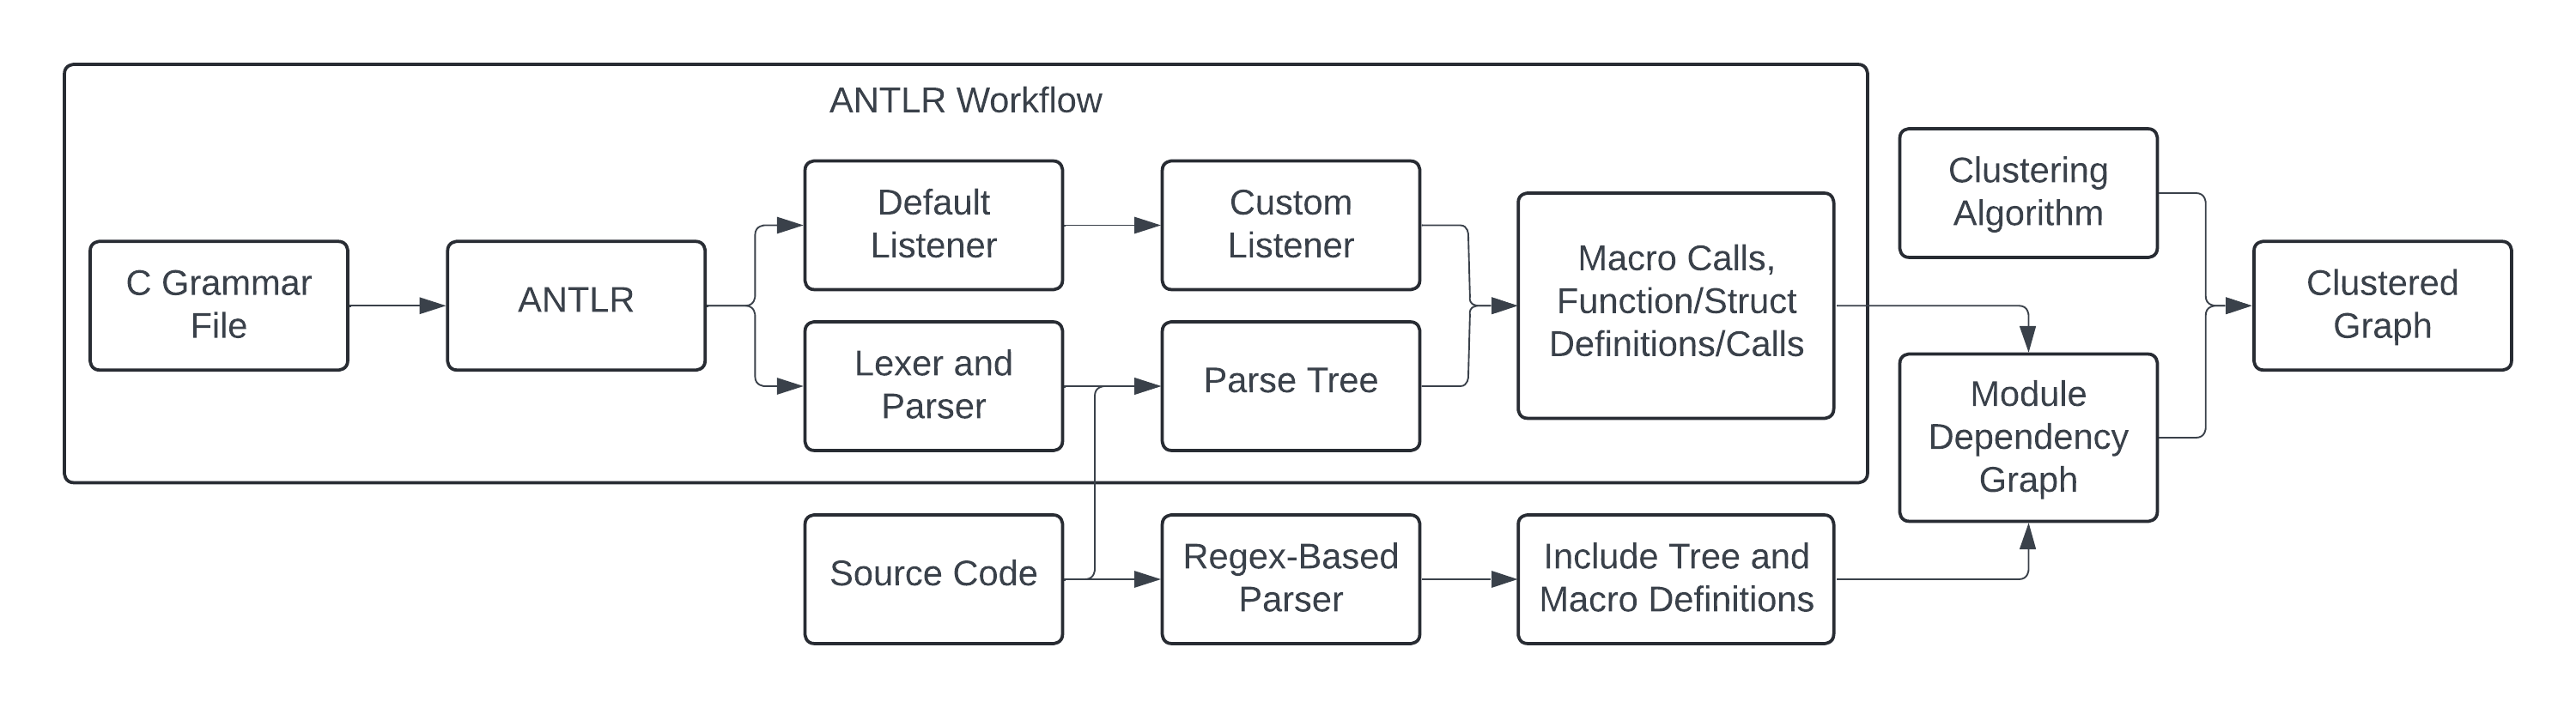
\includegraphics[width=1.0\linewidth]{figures/workflow_diagram.png} \\
    \caption{A diagram of the workflow used for the analysis of HPC code-bases.}
    \label{fig:workflow}
\end{figure*}

\subsection{Graph Construction}
\label{subsec:graph_construction}

The dependency data extracted from each file consisted of the include statements which were used to form the spine of the dependency graph and the declarations and instantiations of dependencies to create the weightings along each edge of the graph. The dependencies of interest were macros, functions, types, structs, global variables, and unions. The include statements and macro definitions were easily extracted from each file with RegEx parsing techniques as they use well-defined pre-processor directives, \#include and \#define respectively, which a regular grammar is more than capable of handling. The macro instantiations and the declarations/instantiations of the other dependency types required a context-sensitive grammar to extract them. ANTLR was chosen for this purpose with the details of the developed workflow being covered in Section \ref{subsec:antlr_workflow}.

For the graph's construction, files were initially chosen as the nodes as they are the fundamental unit that developers work with when partitioning the functional dependencies of their code. Files of interest in the code included *.c files which contain the implementations of code, *.h files which provide the code's interfaces so *.c files can access one another's functions and declarations, and *.inl files which contain inline functions. Inline functions are similar to macros in that they get expanded inline be the compiler to provide speedup benefits as the functions don't need to be called at runtime. Each file node was named by the path of the file relative to the source code directory (e.g. path/to/file.c) in order to ensure unique node names through the graph. After parsing was complete, each of these file nodes contained the file's name, the number of lines in the file, lists of definitions and instantiations of dependencies in the file, and a hash of the files that the node depends on according to the include statements. The lists of dependencies were split into macros and non-macros in order to analyze if there were differences between how each group was utilized across the code-base. The hash of file dependencies used the names of the files that were included as the key and the number of dependencies as the value. The number of dependencies file A had on file B was calculated by taking the list of instantiations in file A, removing the definitions in file A, then counting the number of instances remaining in file A that were defined in file B. This hash was then used to form the edge weightings for the graph.

Initial testing revealed that handling each file independently resulted in scaling issues with respect to the standpoints of algorithm runtime and outputting human-interpretable representations of the results as the code-bases consisted of hundreds of files. This required hierarchical techniques to be employed in order to reduce the total number of nodes in the graph. In order to achieve this, a secondary node type which represented clusters of related nodes was employed. These clusters can be thought of as black-boxes that appear as a single file to other nodes that contains the dependency sums of its component files. In implementation, these nodes simply contain a cluster name and a list of the nodes within the cluster. The cluster names were the last common path shared by the files in the cluster followed by an index to differentiate between clusters under the same directory (e.g. cluster/path:0, cluster/path:1). Since clusters appear as files to other nodes, clusters can also be nested with this method. The requirement for this construction is that any given file can only appear once in the graph meaning that a file cannot be a direct child of two clusters and a file in a cluster cannot appear outside the cluster.

Cluster nodes were used in two instances throughout the experiments: to group together *.c, *.h, and *.inl files of the same name (e.g. path/to/file.c, path/to/file.h, and path/to/file.inl) and to group together algorithm-identified clusters in a given sub-directory of the source code. Figure \ref{fig:graph_example} demonstrates what the network diagrams of the graphs look like for cluster nodes at different levels of the hierarchy. The grouping of files that had the same name except, for their type extension, was done to reduce the total file count of the code-base. These files are tightly coupled in their content by convention which is why this decision was deemed low-risk to the final results. Section \ref{subsec:workloads} provides insight into the effects this decision made on the size of the workloads. Figure \ref{fig:graph_example} a) and b) demonstrate the degree to which reducing the file counts can benefit the interpretability of the results with a) containing 13 nodes and b) containing 29, or a node count reduction of 55\%. The grouping of algorithm-identified clusters allowed for the clustering to happen hierarchically by folder. This means that in the example of file path/to/files/files.ext, files.ext would be hierarchically included in the hierarchical clusters of path/to/files:n, path/to:n, and path:n. This allowed for looking at the dependencies between files at different levels of the code-base's directory structure.

\begin{figure*}[ht]
    \centering
    \begin{tabular}{c c }
        \includegraphics[width=0.48\linewidth]{figures/graph_design_examples/ucp_core_clustered.png}
        & \includegraphics[width=0.48\linewidth]{figures/graph_design_examples/ucp_core.png} \\
        a) ucp/core:0 with file-level clustering.
        & b) ucp/core:0 without file-level clustering. \\
        \includegraphics[width=0.48\linewidth]{figures/graph_design_examples/ucp.png}
        & \includegraphics[width=0.48\linewidth]{figures/graph_design_examples/ucx.png} \\
        c) ucp:0. & d) ucx:0. \\
    \end{tabular}
    \caption{Network diagrams demonstrating the visual representation of the hierarchical clustering graphs of UCX. Note that d) depicts all of UCX so was named after the project as the relative path from the source directory is null.}
    \label{fig:graph_example}
\end{figure*}



\subsection{The ANTLR Workflow}
\label{subsec:antlr_workflow}

In this work we will be using a modified version of ANTLR's default C grammar file. The details of the modifications will be covered later in this section. The tools generated by ANTLR included a lexer, parser, and listener. A lexer is a tool that takes an input string and converts it to a set of tokens in accordance with the rules set out by the grammar file. A parser then takes these tokens and returns a parse tree, also based on the grammar's rules. A parse tree is a tree graph structure that represents the syntactical structure of the parsed file. The leaf nodes are the characters that are directly in the file with the parent nodes defining the semantic context its children fall into. Figure \ref{fig:hello_world} shows an example parse tree for a "Hello world" function using the C grammar. From the parse tree, a breadth-first search can be conducted. The listener instantiates events every time a node in the tree is entered or exited where nothing happens. The user can then customize these events to execute an arbitrary block of code with a context provided as to the location in the tree.

\begin{figure}[ht]
    \centering
    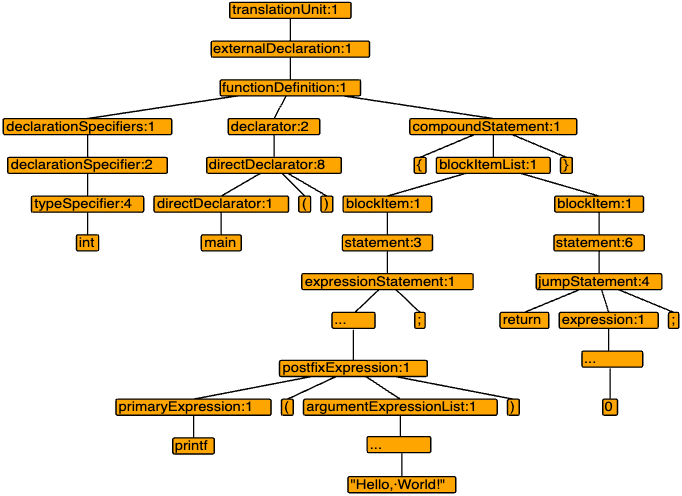
\includegraphics[width=1.0\linewidth]{figures/antlr_hello_world.png} \\
    \caption{An ANTLR parse tree for hello world in C. Note that vertical chains of nested contexts are replaced with "..." for brevity.}
    \label{fig:hello_world}
\end{figure}

In the hello world example in Figure \ref{fig:hello_world}, a user defined block of code could be run every time a directDeclarator context is entered to capture its name if the name exists and the directDeclarator is the grandchild of a functionDefinition. This would result in the name of the function, main, being captured. These types of listener events were defined in the custom listener for this work in order to capture the dependency information for the definitions and instantiations of the types of interest outlined in Section \ref{subsec:graph_construction}. Macros and include statements were covered with regex rather than with the listener as ANTLR's C grammar file doesn't capture pre-processor directives, pre-processor directives are non-semantic in nature as they always are the string which directly follows their directive (\#include and \#define respectively), and it is simpler to use RegEx than to create definitions for them in the grammar files.

As previously noted, the C grammar file provided by ANTLR required modifications in order to be useful for this project. The primary concern was the lack of a definition for macros which, as discussed in Section \ref{sec:intro} and demonstrated in Table \ref{tab:library_metadata} of Section \ref{subsec:workloads}, are a significant component in HPC code-bases. This was a significant undertaking as macros can appear very similar and/or very dis-similar to functions definitions and instantiations. The complexity from this came from making the macro grammar components general enough to cover a plethora of edge cases while also specific enough as to interpret non-macros as macros. Macros can also take in anything as an argument which created more complexities as anything was inclusive of more exotic components such as operators, reserved identifiers, other macros, and function instantiations and declarations. The final grammar file used was not able to remove 100\% of the errors that were encountered, but none of the errors lead to termination conditions and the number of errors in proportion to the size of the code-bases were insignificant as will be explored in Section \ref{subsec:workloads}.


%%%%%%%%%%%%%%%%%%%%%%%%%%%%%%%%%%%%%%%%%%%%%%%%%%%
\subsection{Clustering Algorithms}
\label{subsec:alg_description}

For the clustering algorithms, the methodology used was based on one proposed in prior works on file dependency clustering of code-bases \cite{792498_bunch, 693283_auto_clustering}. This method takes the nodes in the graph as a set that can be partitioned (segmented into non-empty subsets, or clusters, of the graph that collectively span the superset). The goal is to find a partition which best modularizes the code-base as indicated by the maximization of intra-dependencies within a cluster and the minimization of inter-dependencies between clusters. The heuristic used to determine this is dubbed the modularization quality (MQ) of the partition, the math of which is covered in Section \ref{subsec:mq_description}. From the MQ value, algorithms can be used to find the partition that best represents the architecture of the code-base.

Two algorithms were selected to find the partition with the best MQ value for k clusters in the partition. Running a monte-carlo of all possible partitions in the search space was also considered as an option, but it was experimentally determined that this was not feasible from a runtime perspective for a k value over 2. The first algorithm is gradient descent which starts with a randomly generated partition of k clusters where k is user-defined, then checks every possible neighboring partition to find the partition with the best MQ value. A neighboring partition is defined as a partition where all nodes except for one are in the exact same position. As with any gradient descent problem, multiple start points are required to find the best possible partition so each hierarchical set was run for 20 different randomly selected starting partitions. The second algorithm was a genetic algorithm 

Selection of the ideal k value can be done with an elbow-analysis of the curve of a plot with k as the x-axis and MQ as the y-axis. The elbow in the curve indicates the ideal k value for a given graph topology. The issue with this technique is that it is topology-dependent and therefore would require a sweep to be done for every sub-partition independently. As will be seen in Section \ref{sec:results}, the code-bases have over 300 combined sub-partitions that would need this analysis done. This leads to a scaling issue that makes this type of analysis untenable for the purposes of this work in contrast to works in which less hierarchical, and therefore less unique topologies, are considered. The route taken instead was to do static k value selection based on the number of nodes in a partition. The k values were determined experimentally as $k = 1$ for up to 4 nodes in a partition, 2 for up to 6, 3 for up to 15, 4 for up to 24, and 5 for 25 or more.


%%%%%%%%%%%%%%%%%%%%%%%%%%%%%%%%%%%%%%%%%%%%%%%%%%%
\subsection{Modularization Quality}
\label{subsec:mq_description}

Each cluster in a partition has intra-dependencies between the nodes it contains and inter-dependencies with other clusters in the partition. Equation \ref{eqn:intraconnectivity} defines the intra-dependency of cluster i where $\mu$ is the number of intra-dependencies in the cluster and N is the number of nodes in the cluster. Equation \ref{eqn:interconnectivity} similarly defines the inter-dependency between cluster i and cluster j where $\epsilon$ is the number of inter-dependencies between the clusters. Both of these metrics are bounded in the domain of [0,1] where $A_i = 0$ is no relation between files in a cluster, $A_i = 1$ means the cluster is fully connected, $E_{i,j} = 0$ is no dependencies between the clusters, and $E_{i,j} = 1$ means the clusters are fully connected. 

\begin{equation}
    A_i = \dfrac{\mu_i}{N_i^2} \\
    \label{eqn:intraconnectivity}
\end{equation}

\begin{equation}
    E_{ij} =
    \begin{cases}
        0 & i = j \\
        \dfrac{\epsilon_{ij}}{2N_iN_j} & i \ne j \\
    \end{cases}
    \label{eqn:interconnectivity}
\end{equation}

With the goal in mind of attempting to discern the architectural construction of the code-base, the objective is to find the partition which minimizes the inter-dependencies and maximizes the intra-dependencies as these characteristics lead to the most modular grouping of nodes. The modularization quality (MQ) of a partition is a heuristic defined by the inter- and intra-dependencies of the clusters. The bounds of the MQ are [-1, 1] with -1 indicating no cohesion within the clusters and 1 indicating no coupling between the clusters.

\begin{equation}
    MQ =
    \begin{cases}
        \dfrac{1}{k} \sum_{i=1}^{k} A_i - \dfrac{1}{\dfrac{k(k-1)}{2}} \sum_{i,j=1}^{k} E_{i,j} & k > 1 \\
        \dfrac{\epsilon_{ij}}{2N_iN_j} & k = 1 \\
    \end{cases}
    \label{eqn:mq_heuristic}
\end{equation}

The one drawback of the MQ heuristic is that it assumes an unweighted graph. In order to account for this, a simple multiplication factor was added to the inter- and intra-connectivity factors. These modified factors are represented by Equations \ref{eqn:weighted_intra} and \ref{eqn:weighted_inter} respectively where w\_i is the weight of the inbound edges for node i, W is the total weight of all edges in a cluster, and $m_{ij}$ is the weight between two nodes, i and j. The weighted MQ heuristic (WMQ) is identical to Equation \ref{eqn:mq_heuristic} but with WA and WE in place of A and E respectively.

\begin{equation}
    WA_i = \dfrac{w_i\mu_i}{WN_i^2} \\
    \label{eqn:weighted_intra}
\end{equation}

\begin{equation}
    WE_{ij} =
    \begin{cases}
        0 & i = j \\
        \dfrac{m_{ij}}{2N_iN_j} & i \ne j \\
    \end{cases}
    \label{eqn:weighted_inter}
\end{equation}


\subsection{The Middleware Libraries}
\label{subsec:workloads}

%HPC libraries that sit below the applications but above the hardware fall into two primary categories: middleware libraries and communication protocol libraries. Middleware libraries sit directly above the InfiniBand network and bellow the protocol libraries to provide low-level network interfacing all the way down to the hardware. Protocol libraries implement communication standards through the use of these middlewares such as message passing or remote memory access. For this work, we will be looking at running the methodology on middleware libraries as they are the primary focus,

Three middleware libraries were selected for this work, namely Unified Communication-X (UCX), Open Fabrics Interface (OFI), and Sandia National Lab's (SNL's) implementation of Portals4 (Portals). These three were selected as they are the only known open-source HPC middlewares that have been used in production systems. Table \ref{tab:library_metadata} displays an overview of general metrics of interest related to code-base size and composition. The files counts and lines of code are divided by file type in order to give an idea as to their composition. ANTLR error counts are provided for insight into the effectiveness of the C grammar file used. A point of note is that ANTLR errors typically have a cascading effect in that one error will cause an incorrect parsing later on as the context is incorrect which causes another error. The unique file name counts are indicative of how many nodes were removed from the cluster using the same-name hierarchical methods discussed in Section \ref{subsec:graph_construction}. Declaration counts are provided to give an idea of the total number of shared dependencies within the codebase and what proportion of them is macros vs non-macros.

\begin{table*}[ht]
    \centering
    \caption{Metadata on the statistics for each of the code-bases including those related to the size of the code-base and the parsed outputs.}
    \begin{tabular}{|c|c|c|c|c|c|c|c|c|c|c|c|c|}
        \hline
            \multirow{2}{*}{Library} & \multicolumn{4}{c|}{Files} & \multicolumn{4}{c|}{Lines of Code} & ANTLR & Unique File & Macro & Non-Macro \\
        \cline{2-9}
            & All & *.c & *.h & *.inl & All & *.c & *.h & *.inl & Errors & Names & Declarations & Declarations \\
        \hline
        \hline
            UCX & 540 & 253 & 258 & 29 & 201,454 & 133,512 & 58,553 & 9,389 & 901 & 329 & 1222 & 34,176 \\
        \hline
            OFI & 1159 & 697 & 462 & 0 & 541,459 & 424,588 & 116,871 & 0 & 2088 & 1048 & 3702 & 53,708 \\
        \hline
            Portals & 217 & 135 & 82 & 0 & 60,204 & 46,149 & 14,055 & 0 & 177 & 177 & 325 & 6080 \\
        \hline
        %    SOS & 69 & 38 & 23 & 8 & 29,474 & 16,834 & 8,623 & 4017 & 1670 & 60 & 588 & 3196 \\
        %\hline
        %    OpenMPI & 1910 & 1600 & 310 & 0 & 347,772 & 283,853 & 63,919 & 0 & 3567 & 1777 & 965 & 40,548 \\
        %\hline
        \hline
            UCT & 205 & 103 & 98 & 4 & 84,339 & 57,732 & 23,722 & 2,885 & -  & - & 297 & 14,976 \\
        \hline
            UCP & 137 & 71 & 46 & 20 & 67,674 & 47,474 & 14,390 & 5,820 & -  & - & 161 & 13,077 \\
        \hline
            UCS & 198 & 79 & 114 & 5 & 49441 & 283,306 & 20,451 & 684 & -  & - & 764 & 6,123 \\
        \hline
    \end{tabular}
    \label{tab:library_metadata}
\end{table*}


What follows is a description of the three middleware libraries of interest in order to give context for the analyses in Section \ref{subsec:arch_extraction}. Extra analysis is provided for UCX in Section \ref{subsec:ucx_arch} so the description for it is a bit more in-depth as to it's component's inner workings than the other two. Table \ref{tab:library_metadata} also includes a breakdown of the UCX data for each of its individual components.

UCX \cite{ucx_github} is an open-source communication framework developed by NVIDIA with wide-spread adoption in HPC systems and having other proprietary HPC network fabrics being built on top of it \cite{openfabrics_libfabric}. UCX is the most notorious for its code complexity and lack of documentation out of the code-bases selected which is why it was selected for a deeper analysis. UCX has three primary components which are highly interconnected with one another:
\begin{itemize}
    \item Protocols (UCP) - implements high-level protocols (e.g. MPI) to expose the capabilities of UCT to the application
    \item Transport (UCT) - abstracts the hardware architecture to enable communication protocols over the network
    \item Service (UCS) - provides the functionality for implementing portable and efficient utilities with OS bypassing for direct memory management
\end{itemize}

Portals \ref{portals4_repo} is a modular network middleware implementation of the Portals 4 standard \ref{portals4.3} that focuses on providing communication libraries with the tools they need to implement any protocol. The Portals 4 standard was developed by SNL as an alternative to UCX which sought to provide communication libraries with a more sophisticated suite of tool. Portals is a lightweight option that was deployed on systems at US national labs as a proof of concept as to the possibilities of the Portals 4 standard as a middleware. OFI \cite{libfabric_repo} is an implementation of the Portals 4 standard that was deployed by Intel in a collaboration with SNL following Portals' success. It is actively maintained by Intel and used on production systems. Portals in no longer actively maintained as a result of OFI's success.

%\begin{figure*}[ht]
%    \centering
%    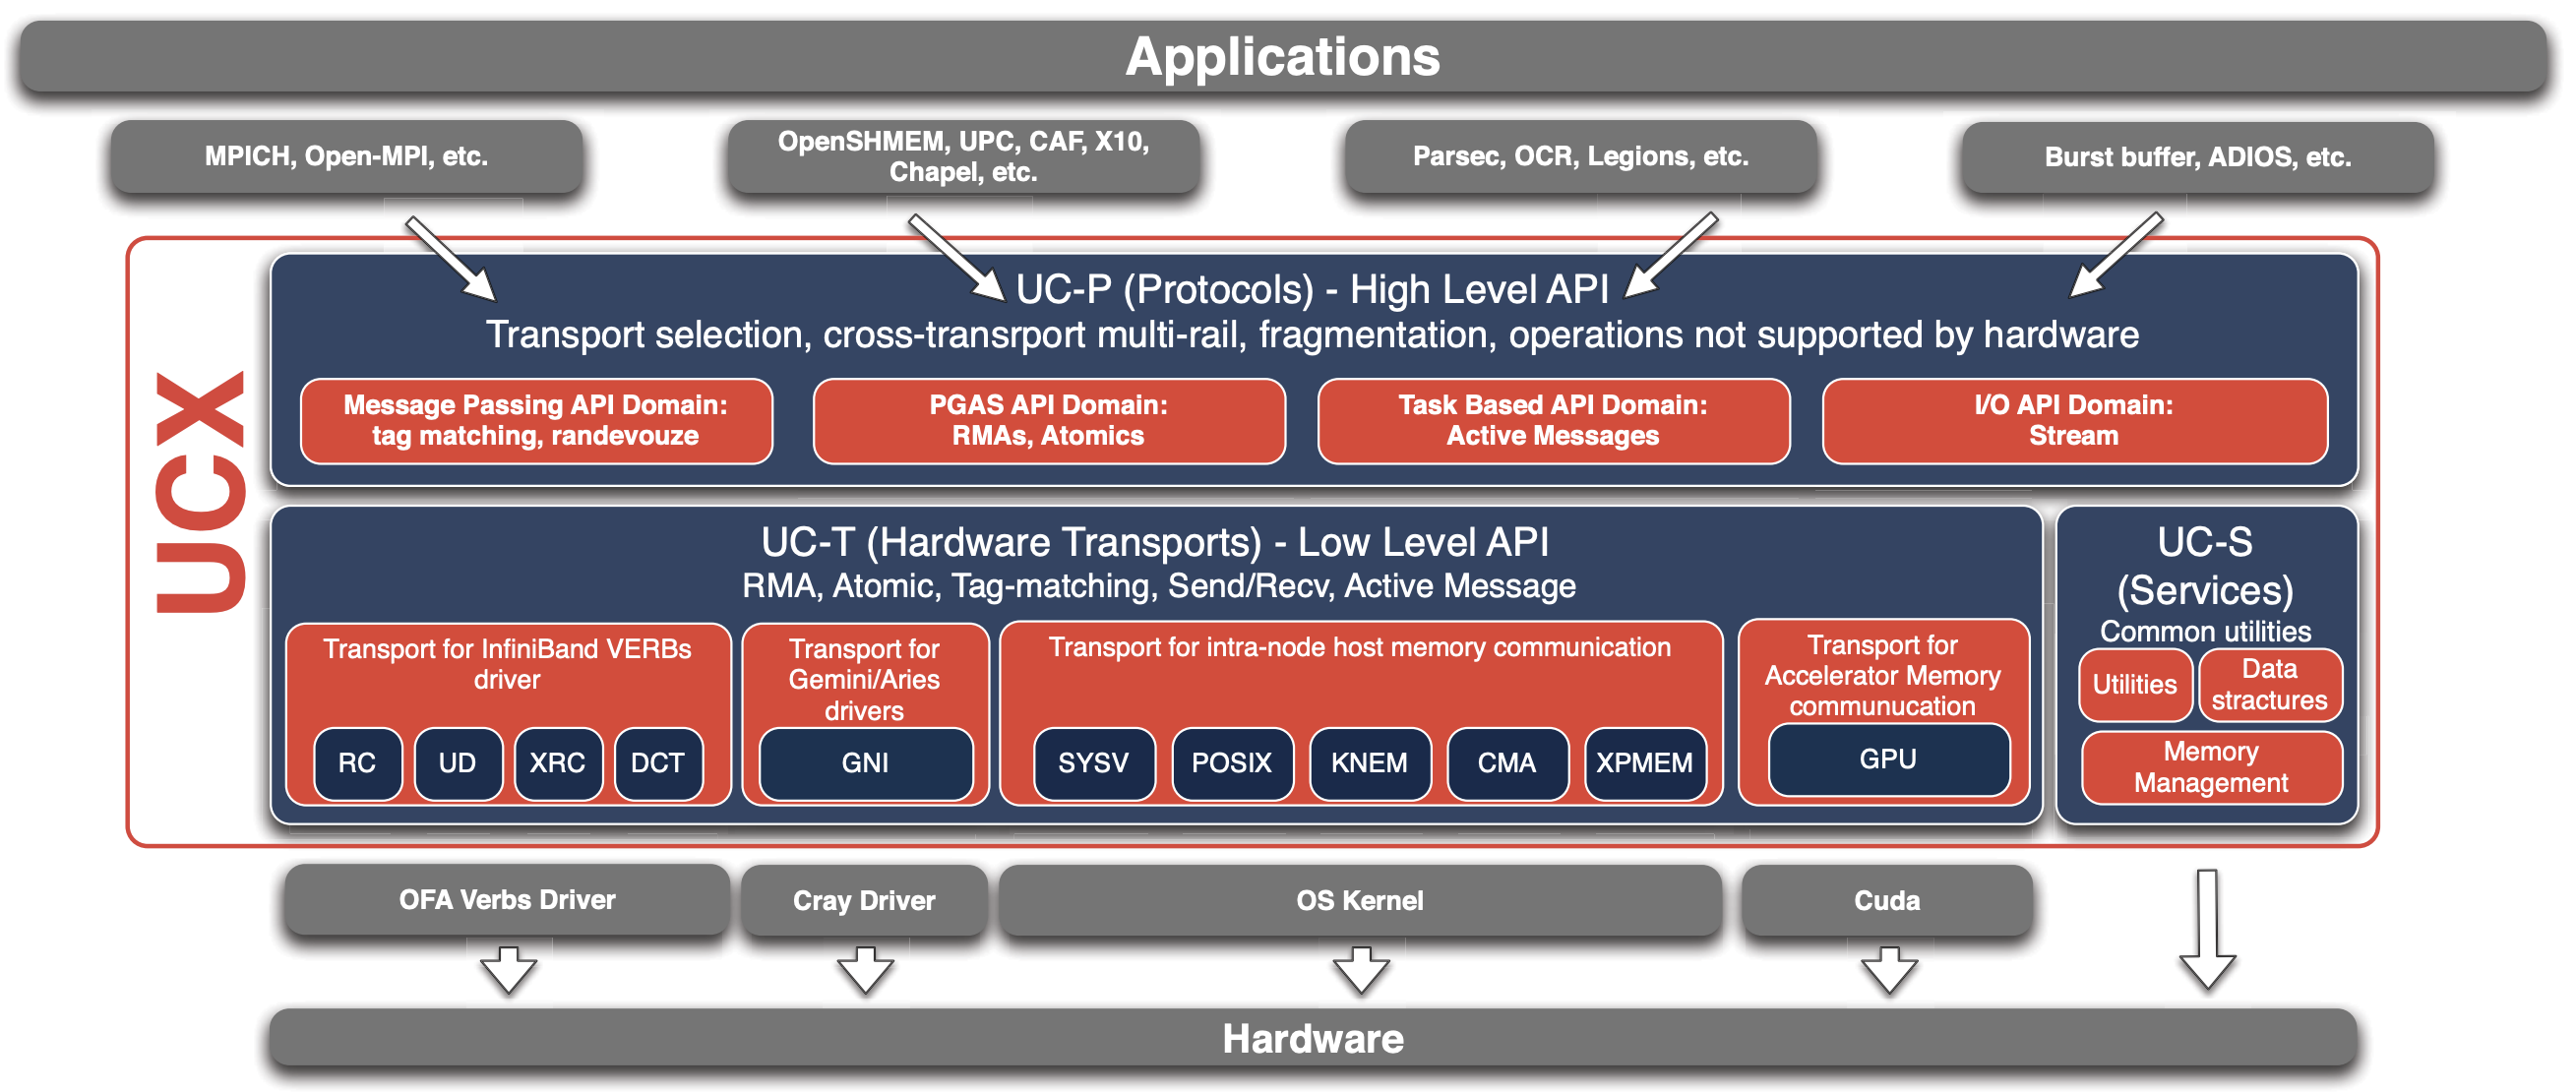
\includegraphics[width=1.0\linewidth]{figures/ucx_structure.png} \\
%    \caption{A high-level overview of the UCX architecture taken from the original paper \cite{ucx_paper}.}
%    \label{fig:ucx_struct}
%\end{figure*}



\section{Research Results}
\label{sec:results}

\begin{table*}[ht]
    \centering
    \caption{Results of running the clustering algorithms on each of the code-bases.}
    \begin{tabular}{|c|c|c|c|c|c|c|}
        \hline
             \multirow{2}{*}{Library} & \multirow{2}{*}{Sub-Partitions} & One-Valued & \multicolumn{2}{c|}{Mean MQ} & \multicolumn{2}{c|}{Mean WMQ} \\
        \cline{4-7}
            & & Sub-Partitions & Gradient & Genetic & Gradient & Genetic \\
        \hline
        \hline
            UCX & 87 & 58 & 0.4425 & 0.4471 & 0.4430 & 0.4479 \\
        \hline
            OFI & 204 & 164 & 0.3738 & 0.3751 & 0.3686 & 0.3708 \\
        \hline
            Portals & 47 & 40 & 0.4471 & 0.4031 & 0.4046 & 0.4390 \\
        \hline
            %SOS & 2 & 0 & 0.4256 & 0.4396 & 0.4401 & 0.4236 \\
        %\hline
        %    OpenMPI & & & & & & \\
        %\hline
        %\hline
        %    UCT & & & & & \\
        %\hline
        %    UCP & & & & & \\
        %\hline
        %    UCS & & & & & \\
        %\hline
    \end{tabular}
    \label{tab:mq_results}
\end{table*}


\begin{figure}[Ht]
    \centering
    \begin{tabular}{c}
        \includegraphics[width=0.96\linewidth]{figures/ucx_analysis/ucp.png} \\
        a) UCP \\
        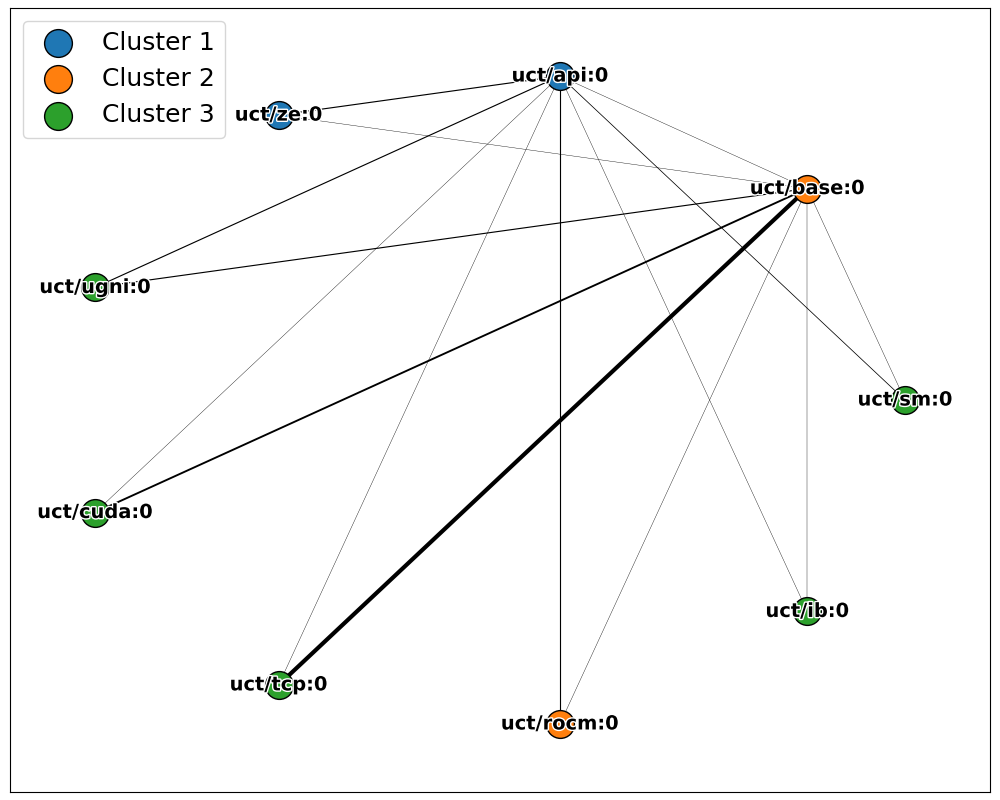
\includegraphics[width=0.96\linewidth]{figures/ucx_analysis/uct.png} \\
        b) UCT \\
        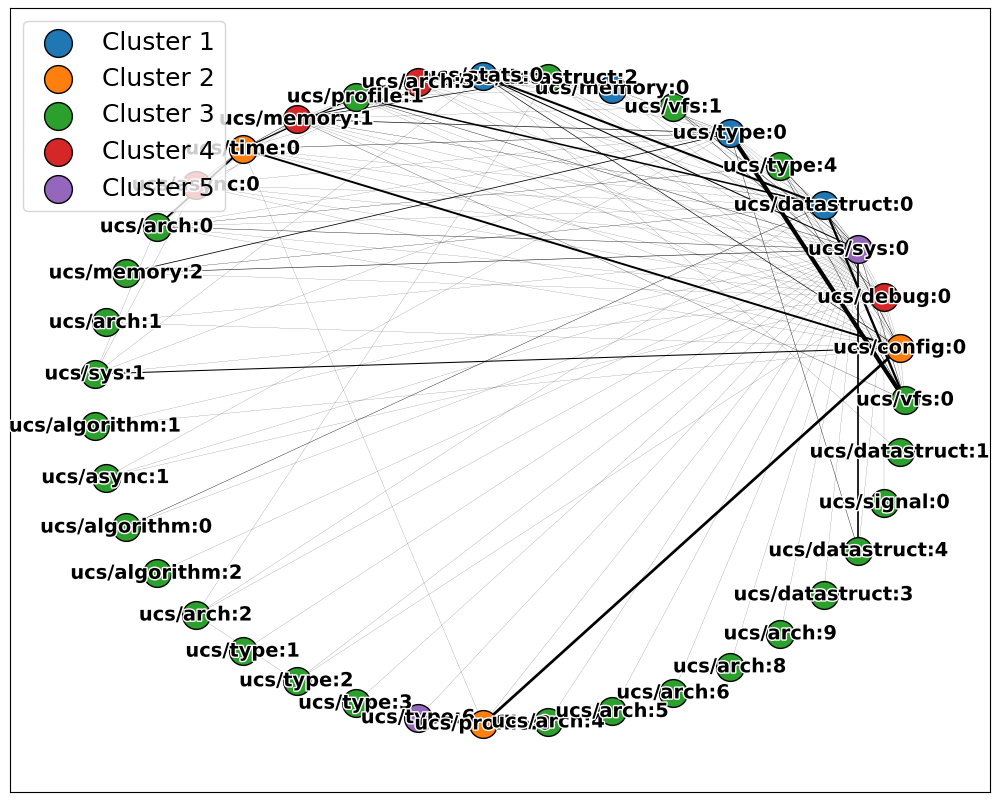
\includegraphics[width=0.96\linewidth]{figures/ucx_analysis/ucs.png} \\
        c) UCS \\
    \end{tabular}
    \caption{Network diagrams for UCX's top-level components.}
    \label{fig:ucx_components}
\end{figure}

This section seeks to answer three research questions (RQs) by analyzing the results of executing the methodology outlined in Section \ref{sec:methodology}. The research questions are:
\begin{enumerate}
    \item Which clustering algorithm results in the lowest mean MQ value across the different HPC code-bases?
    \item Are clustering algorithms useful in extracting the architecture of HPC middleware libraries?
    \item How can the information generated by the proposed methodology be used to help deepen ones understanding of UCX?
\end{enumerate}

RQ1 aims to identify the best clustering algorithm for architecture extraction and will be achieved by quantitatively testing each of the algorithms with MQ and WMQ heuristics for each of the code-bases. RQ2 looks at if the clustering results are useful in extracting architecture patterns on arbitrary HPC libraries in order to check the utility of the methodology proposed in this work. This will be done through a qualitative inspection of the hierarchical clusters that were produced through the methodology's execution on each of the code-bases. RQ3 builds on the results of RQ2 by exploring how the surface-level intuition gained about the architecture can be used to examine the source code in a more informed manner. Only UCX will be explored for RQ3 due to the depth of analysis required and space constraints.
% RQ3 aims to take a deeper dive into the utility of this methodology for developing an understanding of a code-base. 

%%%%%%%%%%%%%%%%%%%%%%%%%%%%%%%%%%%%%%%%%%%%%%%%%%%
\subsection{Algorithm Performance}
\label{subsec:alg_perf}

Both algorithms were run for each of the libraries with both the weighted and unweighted MQ variants. Table \ref{tab:mq_results} show the results of these tests with the best values from 10 random seeds. The number of sub-partitions in the table is the number of partitions that were clustered in order to build the project-level hierarchy. In the example of UCX shown in Figure \ref{fig:graph_example} d), the top level partition is composed of ucp:0, uct:0, ucs:0, and ucs:1. This would count as 4 sub-partitions at the top-level and then be run recursively to determine the sub-partition count for the entire code-base. Since the number of sub-partitions generated are deterministic based on the directory structure and fixed k values, the sub-partition counts are constant across each algorithm. For the mean values, only hierarchical clusters with non-one MQ values were considered as to not skew the results with MQ values that were deterministic rather than generated by the algorithms.

The general results seen in the table are that there is no common trend for which algorithm results in the best MQ value when looking across multiple code-bases. The differences between MQs for algorithms in any given code-bases were also marginal with the greatest difference being Portals with a $(gradient - generic)$ MQ difference of 0.0440 and a WMQ difference of -0.0344. It is an interesting point that, even looking at the MQ and WMQ heuristics for the same code-base, there isn't a consistency in the best performer between the two algorithms. This leads to the conclusion that the performance difference in finding the best MQ values between the two algorithms and the two heuristics is inconsequential. 

%%%%%%%%%%%%%%%%%%%%%%%%%%%%%%%%%%%%%%%%%%%%%%%%%%%
\subsection{Architecture Extraction}
\label{subsec:arch_extraction}

For the UCX library, the components of UCS, UCT, and UCP are heavily dependent on one another with a lot of dependencies that interweave their construction, but each of the components also has their own distinct architecture. Each of the major components of UCX are shown in Figure \ref{fig:ucx_components}, but the components of the other libraries will only be discussed and not be shown due to space restrictions. UCP is focused around its api and core components with core being fully connected to all other components and api primarily servicing the wireup and rma components. UCS is heavily dependent on its datastruct component which services data structures for in-memory processing alongside its sys component which implements the system calls for OS bypassing. UCT is built around its api and base components, similar to UCP, but each of the components only connect to these two which reflects how each component is instantiated based on what hardware is being used.

For the OFI library, the broad architecture that can be extracted from the results are that the "include" directory is where all of the *.h files that connect components are kept. The *.h files in the component directories are primarily for dependencies within the same component (e.g. rdma interface files reference other rdma files directly, but not ucx interface files). At this top level, the primary files that dictate dependencies are ofi\_util.h which bootstraps the communication protocol components and ofi\_enosys.h that connects the hardware-level interactive components such as atomic operation, network endpoint address resolutions, and message tagging.

For the Portals library, there are virtually no dependencies in the code-base. Upon further inspection from a dumping of the dependency graph data, it appears that there are a over 100 *.h files that simply point to their respective *.c files and an equally great number that don't point to any files. The majority of the *.h files that did point to a *.c file were in the runtime component which instantiated system calls. This makes sense as portals is strictly a modular network API that sits directly on IB verbs rather than providing a framework such as UCX or OFI.

Overall, the qualitative analyses of the broad graphical results have proven to be useful in the extraction of broad architectures for each of the HPC libraries. These analyses are not exhaustive of what can be extracted due to space constraints and have only considered the points that are apparent in the network diagrams. The concern with the analyses conducted is that the analytical points related to the architecture that were extracted were dependent exclusively on the dependency weightings between files rather than the automatic clustering of files done by the algorithms. The cluster results provided no helpful insight beyond what was visible in the dependency analysis and attempts at gleaming insight from them were fruitless. These results lead to the conclusion that the use of clustering algorithms were not useful in extracting the architecture of HPC middleware libraries.

%%%%%%%%%%%%%%%%%%%%%%%%%%%%%%%%%%%%%%%%%%%%%%%%%%%
\subsection{UCX Architectural Patterns}
\label{subsec:ucx_arch}

Next is to do a deep-dive into UCX to see what deeper meaning can be extracted when the results from the network diagrams are considered in conjuncture with an analysis of the source code. Starting with UCP, the core component which had a high degree of dependencies to other components was primarily due to the ucp\_ep sub-component which define the endpoint characteristics for the network. This component establishes endpoint control (e.g. instantiation, connection characteristics, protocols, etc.) which is a fundamental aspect of network communications. These files have dependencies utilize the lane protocols from the proto component and the endpoint matching from the wireup component. Further analyses revealed that ucp\_ep is indeed the backbone component for UCP's design which the other components build on top of. For example, stream, rndv, and rma are all protocols that sit on top of the endpoint connection and use core's other sub-components (e.g. workers, buffers, and requests) to execute. The API component also had a notable number of dependencies, but that's primarily due to it being the interface for usage external to UCP which necessitates its inter-dependencies to all externally visible components.

Looking next at the construction of UCS, the datastruct and sys components were prevalent in the initial analysis. The datastruct component has little-to-no internal structure that lends itself to further analysis with pseud-random connections between its sub-components, but it is worth noting that datastruct is the most commonly called component across not only UCS, but UCP and UCP as well. This makes sense as it implements all of the optimized datatypes and how they are managed directly in memory. Switching to the sys component, the sub-component by the same name (i.e. sys/sys) is the most heavily utilized. This appears to be due to it being where the system calls are primarily implemented with the other sub-components acting as supports for it. It is also worth noting that UCS doesn't have an API component unlike UCP and UCT. This makes sense as UCS has been seen here to primarily implement fundamental building blocks such as system calls and data structures which UCP and UCT can utilize rather than providing services such as the endpoint connections seen in the UCP analysis.

Finally looking at UCT, the base component immediately appears to be the backbone of the design with other components being connected to it exclusively. The API component is the notable exception to this, but due to the reasons mentioned in the UCP analysis is deemed to be not of any greater note. Looking at the base component's construction, the iface sub-component is the most utilized as it provides a template for the transport interface model that's being used by other components (i.e. cuda, ib, rocm, tcp, etc.). Further analysis revealed that this is common for the other sub-components of the core module as well as the component that is implemented depending on the target hardware drivers specified at compilation. For example, if CUDA drivers and InfiniBand are detected for hardware support then the cuda and ib components of the transport layer are built over the base template at compile time.



\section{Threats to Validity}
\label{sec:validity}

%\cus{reconsider this whole section once everything else is ironed out}

The ANTLR workflow hinges on the quality of the grammar file which is has proven issues as evident by the error counts in Table \ref{tab:library_metadata}. This is due to the complexity in designing a grammar file that is language-complete which necessitated it being outside the scope of this work due to time constraints. The fine-tuning of the grammar file was done with UCX as it was the code-base that was most heavily analyzed in this work to mitigate the impact to the depth-based analysis results. The resulting error rate per lines of code for UCX was able to be brought down to 0.45\%. The ANTLR error results for the other libraries were 0.39\% for OFI 0.29\% for Portals. An error rate of zero is always desirable, but all three libraries having error rates below half a percent was acceptable as it is a marginal proportion and is not believed to have influenced the overall results.

There is an ever-present concern with comparative works as to if the number of items under study is sufficient. In the case of the number of algorithms analyzed two were selected (and a third considered as detailed in Section \ref{subsec:alg_description}), in order to see if a drastic difference was noticeable. Two heuristics were also considered, MQ and WMQ, which adds an additional dimension of variation to the algorithms. The results presented in Section \ref{subsec:alg_perf} demonstrated that there was no consistent performance difference between the algorithms which indicates that a drastically different approach, such as a fundamentally different heuristic or a ML-based clustering, could be a better point for comparison. The other point of varying the number of elements under study is the number of code-bases analyzed. The primary goal of this work was to analyze HPC middlewares, of which three were analyzed to provide variety with more not being available as was noted in Section \ref{subsec:workloads}.
%More were not available for analysis as these are the only open-source HPC middleware solutions available.

In order to test the portability of the methodology beyond HPC middlewares, four additional open-souce C-based code-bases were also tested. The results of these tests were omitted from this work in order to not detract from the focus on HPC middleware libraries. The first two codes tested were HPC communication libraries as they provided tests in the same field but outside of the middlewares niche. The communication libraries selected for this study were namely the OpenMPI implementation of the MPI standard and SNL's implementation of OpenSHMEM (SOS), a shared memory library for remote direct memory accessing (RDMA). The other two codes were applications rather than libraries: LAMMPS \ref{lammps_repository}, a molecular dynamics simulator, and the Apache HTTP server \ref{apache_httpd}. The preliminary numbers confidently pointed to there being no reason to believe that the domain-specificity of the code-base used changes the outcome of the methodology with the limitation being that the codes must be written in C. The one interesting point was that the hierarchical methods used were targeted at the hierarchical code topology of UCX as that's the code-base it was developed on. This means that the results, although still valid representations, could be subject to sub-optimalities in the way the data is represented in the network diagrams. OpenMPI was one such example of this due to the relatively flat directory structure of its codebase with very few subdirectories for component separation.

The two possible points of contention directly related to design choices in the methodology were the k-value selections and the hierarchical analysis methods used. The k-value selection was determined in an ad-hoc experimental process with UCX exclusively and then applied to the other code-bases without further modification. More sophisticated methods such as an elbow-analysis of what k values resulted in diminishing returns were considered, but the resulting MQ and WMQ differences found between different k value configurations were found to only be marginal. This combined with time constraints diminished the priority of a formal k analysis as it is believed it would not effect the final results in any admissible way. As for the hierarchical techniques, there is the possibility that, as mentioned previously with the analysis of non-middleware code-bases, there are certain topologies of code structuring that benefit less from these methods. This was not the case for the codes analyzed and therefore did not effect the outcomes of the work presented, but does pose a generalization issue that would need to be addressed if this methodology were to be executed on other code-bases.

%The fundamental limitation of this work is dictated by the nature of the goal which is that no level of static analysis of the middlewares will provide insight into how they will perform on a given system. This comes back to the points made in Section \ref{sec:intro} about how static analysis of these code-bases typically follow compiler-based options as they allow the expansion of pre-processor directives. This is diametrically opposed to the goals of this work which are to deepen the users understanding of how the source code is written in order to gain insight into the architecture.



\section{Conclusions and Future Work}
\label{sec:conclusions}

This work presented a methodology for extracting dependency graphs from code-bases written in C for the purposes of source code architecture extraction to further new developers understanding of complex codes. The methodology included a combination of ANTLR and RegEx to extract dependency graph, two algorithms for cluster detection in the graph using weighted and unweighted heuristics, and the presentation of the data in network diagrams that display the code-bases topology in a hierarchical manner for ease of analysis. The applications explored through this workflow were specific to the area of HPC middlewares as they are notorious for high levels of complexity and a lack of documentation, but the generalization of the solution was tested in preliminary to ensure the methodology was sound for all C-based codes. The results of testing the methodology proved that the clustering algorithms did not reveal any useful information about the underlying code-bases, but the network diagram representations of the weighted graphs were very helpful in the analysis of the code-bases as was seen through the in-depth analysis of one of the test codes.

Future work should seek to look at alternative methodologies for architecture extraction as the hierarchical clustering component presented in this work did not produce insightful results. Possible alternative methodologies in order of decreasing similarity to this work include trying different hierarchical organization methods to represent the codes differently for algorithm input, using a neural network instead of traditional algorithms to see if alternative patterns can be detected, and using an LLM-based workflow for more context-aware architecture analysis. Since the network diagrams were useful for the analysis of codes, further development should also be sought in that avenue. A tool with an interactive GUI could be developed to allow a better exploration of the weighted dependencies. The specific features such a tool could provide that isn't available in existing solutions would need to be evaluated in more depth, but the general value proposition could be a new way to view code hierarchies to give more context as their weighted dependency structure.

%but the generally offering could be to provide more context to the codes under study and allow the user to put the hierarchies in more context of the overall code-base than can be represented in a static image.

%This tool could provide more context to the codes under study and allow the user to put the hierarchies in more context of the overall code-base than can be represented in a static image.

%This paper outlined a course project proposal for ELEC 876. The proposed project aims to gain an understanding of how UCX, a middleware framework for network communication standards in HPC, is structured and operates. This understanding will be gained by generating an AST of the component pieces of UCX, and UCX in it's entirety, using C-language lexers and parsers generated with ANTLR and a custom parsing script. The AST will then be analyzed using clustering algorithms to traverse the tree and identify patterns within the code, both at the component and holistic levels. The intuition gained from the pattern identification along with the other representations of UCX available will be used to develop some form of documentation for how the code is structured and operates. This will be useful to many people in the HPC community who develop application interfaces such as MPI as it will give them a better understanding about how the middleware is used to interact with the network hardware.


\bibliographystyle{IEEEtran}
\bibliography{bibliography}

\end{document}

%SUMMARY
